% Created by tikzDevice version 0.6.2-92-0ad2792 on 2013-03-31 12:41:54
% !TEX encoding = UTF-8 Unicode
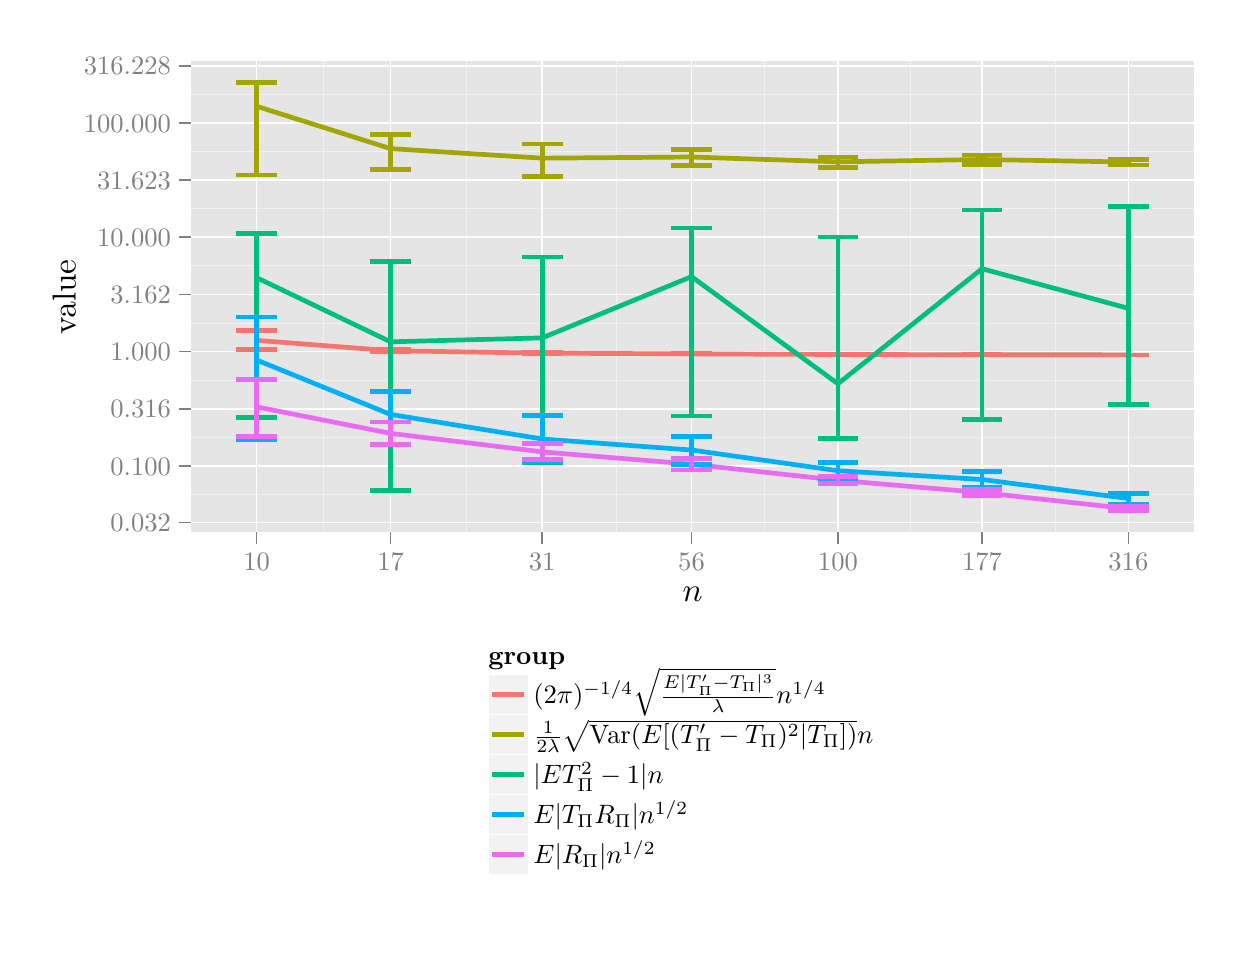
\begin{tikzpicture}[x=1pt,y=1pt]
\definecolor[named]{fillColor}{rgb}{1.00,1.00,1.00}
\path[use as bounding box,fill=fillColor,fill opacity=0.00] (0,0) rectangle (433.62,325.21);
\begin{scope}
\path[clip] (  0.00,  0.00) rectangle (433.62,325.21);
\definecolor[named]{drawColor}{rgb}{1.00,1.00,1.00}
\definecolor[named]{fillColor}{rgb}{1.00,1.00,1.00}

\path[draw=drawColor,line width= 0.6pt,line join=round,line cap=round,fill=fillColor] (  0.00,  0.00) rectangle (433.62,325.21);
\end{scope}
\begin{scope}
\path[clip] ( 58.88,142.81) rectangle (421.57,313.17);
\definecolor[named]{fillColor}{rgb}{0.90,0.90,0.90}

\path[fill=fillColor] ( 58.88,142.81) rectangle (421.57,313.17);
\definecolor[named]{drawColor}{rgb}{0.95,0.95,0.95}

\path[draw=drawColor,line width= 0.3pt,line join=round] ( 58.88,156.64) --
	(421.57,156.64);

\path[draw=drawColor,line width= 0.3pt,line join=round] ( 58.88,177.18) --
	(421.57,177.18);

\path[draw=drawColor,line width= 0.3pt,line join=round] ( 58.88,197.84) --
	(421.57,197.84);

\path[draw=drawColor,line width= 0.3pt,line join=round] ( 58.88,218.50) --
	(421.57,218.50);

\path[draw=drawColor,line width= 0.3pt,line join=round] ( 58.88,239.15) --
	(421.57,239.15);

\path[draw=drawColor,line width= 0.3pt,line join=round] ( 58.88,259.81) --
	(421.57,259.81);

\path[draw=drawColor,line width= 0.3pt,line join=round] ( 58.88,280.46) --
	(421.57,280.46);

\path[draw=drawColor,line width= 0.3pt,line join=round] ( 58.88,301.12) --
	(421.57,301.12);

\path[draw=drawColor,line width= 0.3pt,line join=round] (106.92,142.81) --
	(106.92,313.17);

\path[draw=drawColor,line width= 0.3pt,line join=round] (158.53,142.81) --
	(158.53,313.17);

\path[draw=drawColor,line width= 0.3pt,line join=round] (212.91,142.81) --
	(212.91,313.17);

\path[draw=drawColor,line width= 0.3pt,line join=round] (266.33,142.81) --
	(266.33,313.17);

\path[draw=drawColor,line width= 0.3pt,line join=round] (318.82,142.81) --
	(318.82,313.17);

\path[draw=drawColor,line width= 0.3pt,line join=round] (371.30,142.81) --
	(371.30,313.17);
\definecolor[named]{drawColor}{rgb}{1.00,1.00,1.00}

\path[draw=drawColor,line width= 0.6pt,line join=round] ( 58.88,146.42) --
	(421.57,146.42);

\path[draw=drawColor,line width= 0.6pt,line join=round] ( 58.88,166.86) --
	(421.57,166.86);

\path[draw=drawColor,line width= 0.6pt,line join=round] ( 58.88,187.50) --
	(421.57,187.50);

\path[draw=drawColor,line width= 0.6pt,line join=round] ( 58.88,208.17) --
	(421.57,208.17);

\path[draw=drawColor,line width= 0.6pt,line join=round] ( 58.88,228.82) --
	(421.57,228.82);

\path[draw=drawColor,line width= 0.6pt,line join=round] ( 58.88,249.48) --
	(421.57,249.48);

\path[draw=drawColor,line width= 0.6pt,line join=round] ( 58.88,270.13) --
	(421.57,270.13);

\path[draw=drawColor,line width= 0.6pt,line join=round] ( 58.88,290.79) --
	(421.57,290.79);

\path[draw=drawColor,line width= 0.6pt,line join=round] ( 58.88,311.44) --
	(421.57,311.44);

\path[draw=drawColor,line width= 0.6pt,line join=round] ( 82.72,142.81) --
	( 82.72,313.17);

\path[draw=drawColor,line width= 0.6pt,line join=round] (131.13,142.81) --
	(131.13,313.17);

\path[draw=drawColor,line width= 0.6pt,line join=round] (185.93,142.81) --
	(185.93,313.17);

\path[draw=drawColor,line width= 0.6pt,line join=round] (239.88,142.81) --
	(239.88,313.17);

\path[draw=drawColor,line width= 0.6pt,line join=round] (292.78,142.81) --
	(292.78,313.17);

\path[draw=drawColor,line width= 0.6pt,line join=round] (344.86,142.81) --
	(344.86,313.17);

\path[draw=drawColor,line width= 0.6pt,line join=round] (397.74,142.81) --
	(397.74,313.17);
\definecolor[named]{drawColor}{rgb}{0.97,0.46,0.43}

\path[draw=drawColor,line width= 1.7pt,line join=round] ( 82.72,212.23) --
	(131.13,208.47) --
	(185.93,207.59) --
	(239.88,207.33) --
	(292.78,207.11) --
	(344.86,207.03) --
	(397.74,206.97);
\definecolor[named]{drawColor}{rgb}{0.64,0.65,0.00}

\path[draw=drawColor,line width= 1.7pt,line join=round] ( 82.72,296.81) --
	(131.13,281.50) --
	(185.93,278.05) --
	(239.88,278.47) --
	(292.78,276.73) --
	(344.86,277.57) --
	(397.74,276.65);
\definecolor[named]{drawColor}{rgb}{0.00,0.75,0.49}

\path[draw=drawColor,line width= 1.7pt,line join=round] ( 82.72,234.87) --
	(131.13,211.69) --
	(185.93,213.11) --
	(239.88,235.24) --
	(292.78,196.53) --
	(344.86,238.11) --
	(397.74,223.78);
\definecolor[named]{drawColor}{rgb}{0.00,0.69,0.96}

\path[draw=drawColor,line width= 1.7pt,line join=round] ( 82.72,205.12) --
	(131.13,185.45) --
	(185.93,176.58) --
	(239.88,172.59) --
	(292.78,165.11) --
	(344.86,161.94) --
	(397.74,155.08);
\definecolor[named]{drawColor}{rgb}{0.91,0.42,0.95}

\path[draw=drawColor,line width= 1.7pt,line join=round] ( 82.72,188.19) --
	(131.13,178.60) --
	(185.93,171.91) --
	(239.88,167.48) --
	(292.78,161.66) --
	(344.86,157.21) --
	(397.74,151.36);
\definecolor[named]{drawColor}{rgb}{0.97,0.46,0.43}

\path[draw=drawColor,line width= 1.7pt,line join=round] ( 75.37,215.79) --
	( 90.07,215.79);

\path[draw=drawColor,line width= 1.7pt,line join=round] ( 82.72,215.79) --
	( 82.72,209.03);

\path[draw=drawColor,line width= 1.7pt,line join=round] ( 75.37,209.03) --
	( 90.07,209.03);

\path[draw=drawColor,line width= 1.7pt,line join=round] (123.78,209.01) --
	(138.48,209.01);

\path[draw=drawColor,line width= 1.7pt,line join=round] (131.13,209.01) --
	(131.13,207.96);

\path[draw=drawColor,line width= 1.7pt,line join=round] (123.78,207.96) --
	(138.48,207.96);

\path[draw=drawColor,line width= 1.7pt,line join=round] (178.58,207.78) --
	(193.28,207.78);

\path[draw=drawColor,line width= 1.7pt,line join=round] (185.93,207.78) --
	(185.93,207.43);

\path[draw=drawColor,line width= 1.7pt,line join=round] (178.58,207.43) --
	(193.28,207.43);

\path[draw=drawColor,line width= 1.7pt,line join=round] (232.53,207.40) --
	(247.23,207.40);

\path[draw=drawColor,line width= 1.7pt,line join=round] (239.88,207.40) --
	(239.88,207.26);

\path[draw=drawColor,line width= 1.7pt,line join=round] (232.53,207.26) --
	(247.23,207.26);

\path[draw=drawColor,line width= 1.7pt,line join=round] (285.42,207.14) --
	(300.13,207.14);

\path[draw=drawColor,line width= 1.7pt,line join=round] (292.78,207.14) --
	(292.78,207.09);

\path[draw=drawColor,line width= 1.7pt,line join=round] (285.42,207.09) --
	(300.13,207.09);

\path[draw=drawColor,line width= 1.7pt,line join=round] (337.51,207.04) --
	(352.22,207.04);

\path[draw=drawColor,line width= 1.7pt,line join=round] (344.86,207.04) --
	(344.86,207.01);

\path[draw=drawColor,line width= 1.7pt,line join=round] (337.51,207.01) --
	(352.22,207.01);

\path[draw=drawColor,line width= 1.7pt,line join=round] (390.39,206.98) --
	(405.09,206.98);

\path[draw=drawColor,line width= 1.7pt,line join=round] (397.74,206.98) --
	(397.74,206.97);

\path[draw=drawColor,line width= 1.7pt,line join=round] (390.39,206.97) --
	(405.09,206.97);
\definecolor[named]{drawColor}{rgb}{0.64,0.65,0.00}

\path[draw=drawColor,line width= 1.7pt,line join=round] ( 75.37,305.43) --
	( 90.07,305.43);

\path[draw=drawColor,line width= 1.7pt,line join=round] ( 82.72,305.43) --
	( 82.72,272.00);

\path[draw=drawColor,line width= 1.7pt,line join=round] ( 75.37,272.00) --
	( 90.07,272.00);

\path[draw=drawColor,line width= 1.7pt,line join=round] (123.78,286.57) --
	(138.48,286.57);

\path[draw=drawColor,line width= 1.7pt,line join=round] (131.13,286.57) --
	(131.13,273.88);

\path[draw=drawColor,line width= 1.7pt,line join=round] (123.78,273.88) --
	(138.48,273.88);

\path[draw=drawColor,line width= 1.7pt,line join=round] (178.58,283.20) --
	(193.28,283.20);

\path[draw=drawColor,line width= 1.7pt,line join=round] (185.93,283.20) --
	(185.93,271.44);

\path[draw=drawColor,line width= 1.7pt,line join=round] (178.58,271.44) --
	(193.28,271.44);

\path[draw=drawColor,line width= 1.7pt,line join=round] (232.53,281.15) --
	(247.23,281.15);

\path[draw=drawColor,line width= 1.7pt,line join=round] (239.88,281.15) --
	(239.88,275.41);

\path[draw=drawColor,line width= 1.7pt,line join=round] (232.53,275.41) --
	(247.23,275.41);

\path[draw=drawColor,line width= 1.7pt,line join=round] (285.42,278.48) --
	(300.13,278.48);

\path[draw=drawColor,line width= 1.7pt,line join=round] (292.78,278.48) --
	(292.78,274.78);

\path[draw=drawColor,line width= 1.7pt,line join=round] (285.42,274.78) --
	(300.13,274.78);

\path[draw=drawColor,line width= 1.7pt,line join=round] (337.51,279.20) --
	(352.22,279.20);

\path[draw=drawColor,line width= 1.7pt,line join=round] (344.86,279.20) --
	(344.86,275.70);

\path[draw=drawColor,line width= 1.7pt,line join=round] (337.51,275.70) --
	(352.22,275.70);

\path[draw=drawColor,line width= 1.7pt,line join=round] (390.39,277.66) --
	(405.09,277.66);

\path[draw=drawColor,line width= 1.7pt,line join=round] (397.74,277.66) --
	(397.74,275.55);

\path[draw=drawColor,line width= 1.7pt,line join=round] (390.39,275.55) --
	(405.09,275.55);
\definecolor[named]{drawColor}{rgb}{0.00,0.75,0.49}

\path[draw=drawColor,line width= 1.7pt,line join=round] ( 75.37,250.71) --
	( 90.07,250.71);

\path[draw=drawColor,line width= 1.7pt,line join=round] ( 82.72,250.71) --
	( 82.72,184.35);

\path[draw=drawColor,line width= 1.7pt,line join=round] ( 75.37,184.35) --
	( 90.07,184.35);

\path[draw=drawColor,line width= 1.7pt,line join=round] (123.78,240.65) --
	(138.48,240.65);

\path[draw=drawColor,line width= 1.7pt,line join=round] (131.13,240.65) --
	(131.13,157.85);

\path[draw=drawColor,line width= 1.7pt,line join=round] (123.78,157.85) --
	(138.48,157.85);

\path[draw=drawColor,line width= 1.7pt,line join=round] (178.58,242.36) --
	(193.28,242.36);

\path[draw=drawColor,line width= 1.7pt,line join=round] (185.93,242.36) --
	(185.93,168.02);

\path[draw=drawColor,line width= 1.7pt,line join=round] (178.58,168.02) --
	(193.28,168.02);

\path[draw=drawColor,line width= 1.7pt,line join=round] (232.53,252.82) --
	(247.23,252.82);

\path[draw=drawColor,line width= 1.7pt,line join=round] (239.88,252.82) --
	(239.88,184.90);

\path[draw=drawColor,line width= 1.7pt,line join=round] (232.53,184.90) --
	(247.23,184.90);

\path[draw=drawColor,line width= 1.7pt,line join=round] (285.42,249.54) --
	(300.13,249.54);

\path[draw=drawColor,line width= 1.7pt,line join=round] (292.78,249.54) --
	(292.78,176.72);

\path[draw=drawColor,line width= 1.7pt,line join=round] (285.42,176.72) --
	(300.13,176.72);

\path[draw=drawColor,line width= 1.7pt,line join=round] (337.51,259.28) --
	(352.22,259.28);

\path[draw=drawColor,line width= 1.7pt,line join=round] (344.86,259.28) --
	(344.86,183.59);

\path[draw=drawColor,line width= 1.7pt,line join=round] (337.51,183.59) --
	(352.22,183.59);

\path[draw=drawColor,line width= 1.7pt,line join=round] (390.39,260.67) --
	(405.09,260.67);

\path[draw=drawColor,line width= 1.7pt,line join=round] (397.74,260.67) --
	(397.74,189.01);

\path[draw=drawColor,line width= 1.7pt,line join=round] (390.39,189.01) --
	(405.09,189.01);
\definecolor[named]{drawColor}{rgb}{0.00,0.69,0.96}

\path[draw=drawColor,line width= 1.7pt,line join=round] ( 75.37,220.63) --
	( 90.07,220.63);

\path[draw=drawColor,line width= 1.7pt,line join=round] ( 82.72,220.63) --
	( 82.72,176.45);

\path[draw=drawColor,line width= 1.7pt,line join=round] ( 75.37,176.45) --
	( 90.07,176.45);

\path[draw=drawColor,line width= 1.7pt,line join=round] (123.78,193.86) --
	(138.48,193.86);

\path[draw=drawColor,line width= 1.7pt,line join=round] (131.13,193.86) --
	(131.13,174.67);

\path[draw=drawColor,line width= 1.7pt,line join=round] (123.78,174.67) --
	(138.48,174.67);

\path[draw=drawColor,line width= 1.7pt,line join=round] (178.58,185.02) --
	(193.28,185.02);

\path[draw=drawColor,line width= 1.7pt,line join=round] (185.93,185.02) --
	(185.93,168.34);

\path[draw=drawColor,line width= 1.7pt,line join=round] (178.58,168.34) --
	(193.28,168.34);

\path[draw=drawColor,line width= 1.7pt,line join=round] (232.53,177.45) --
	(247.23,177.45);

\path[draw=drawColor,line width= 1.7pt,line join=round] (239.88,177.45) --
	(239.88,167.34);

\path[draw=drawColor,line width= 1.7pt,line join=round] (232.53,167.34) --
	(247.23,167.34);

\path[draw=drawColor,line width= 1.7pt,line join=round] (285.42,168.13) --
	(300.13,168.13);

\path[draw=drawColor,line width= 1.7pt,line join=round] (292.78,168.13) --
	(292.78,161.90);

\path[draw=drawColor,line width= 1.7pt,line join=round] (285.42,161.90) --
	(300.13,161.90);

\path[draw=drawColor,line width= 1.7pt,line join=round] (337.51,164.95) --
	(352.22,164.95);

\path[draw=drawColor,line width= 1.7pt,line join=round] (344.86,164.95) --
	(344.86,158.98);

\path[draw=drawColor,line width= 1.7pt,line join=round] (337.51,158.98) --
	(352.22,158.98);

\path[draw=drawColor,line width= 1.7pt,line join=round] (390.39,156.99) --
	(405.09,156.99);

\path[draw=drawColor,line width= 1.7pt,line join=round] (397.74,156.99) --
	(397.74,153.12);

\path[draw=drawColor,line width= 1.7pt,line join=round] (390.39,153.12) --
	(405.09,153.12);
\definecolor[named]{drawColor}{rgb}{0.91,0.42,0.95}

\path[draw=drawColor,line width= 1.7pt,line join=round] ( 75.37,198.11) --
	( 90.07,198.11);

\path[draw=drawColor,line width= 1.7pt,line join=round] ( 82.72,198.11) --
	( 82.72,177.60);

\path[draw=drawColor,line width= 1.7pt,line join=round] ( 75.37,177.60) --
	( 90.07,177.60);

\path[draw=drawColor,line width= 1.7pt,line join=round] (123.78,182.73) --
	(138.48,182.73);

\path[draw=drawColor,line width= 1.7pt,line join=round] (131.13,182.73) --
	(131.13,174.52);

\path[draw=drawColor,line width= 1.7pt,line join=round] (123.78,174.52) --
	(138.48,174.52);

\path[draw=drawColor,line width= 1.7pt,line join=round] (178.58,175.06) --
	(193.28,175.06);

\path[draw=drawColor,line width= 1.7pt,line join=round] (185.93,175.06) --
	(185.93,169.10);

\path[draw=drawColor,line width= 1.7pt,line join=round] (178.58,169.10) --
	(193.28,169.10);

\path[draw=drawColor,line width= 1.7pt,line join=round] (232.53,169.53) --
	(247.23,169.53);

\path[draw=drawColor,line width= 1.7pt,line join=round] (239.88,169.53) --
	(239.88,165.42);

\path[draw=drawColor,line width= 1.7pt,line join=round] (232.53,165.42) --
	(247.23,165.42);

\path[draw=drawColor,line width= 1.7pt,line join=round] (285.42,162.96) --
	(300.13,162.96);

\path[draw=drawColor,line width= 1.7pt,line join=round] (292.78,162.96) --
	(292.78,160.37);

\path[draw=drawColor,line width= 1.7pt,line join=round] (285.42,160.37) --
	(300.13,160.37);

\path[draw=drawColor,line width= 1.7pt,line join=round] (337.51,158.45) --
	(352.22,158.45);

\path[draw=drawColor,line width= 1.7pt,line join=round] (344.86,158.45) --
	(344.86,156.04);

\path[draw=drawColor,line width= 1.7pt,line join=round] (337.51,156.04) --
	(352.22,156.04);

\path[draw=drawColor,line width= 1.7pt,line join=round] (390.39,152.16) --
	(405.09,152.16);

\path[draw=drawColor,line width= 1.7pt,line join=round] (397.74,152.16) --
	(397.74,150.56);

\path[draw=drawColor,line width= 1.7pt,line join=round] (390.39,150.56) --
	(405.09,150.56);
\end{scope}
\begin{scope}
\path[clip] (  0.00,  0.00) rectangle (433.62,325.21);
\definecolor[named]{drawColor}{rgb}{0.50,0.50,0.50}

\node[text=drawColor,anchor=base east,inner sep=0pt, outer sep=0pt, scale=  0.96] at ( 51.77,143.11) {0.032};

\node[text=drawColor,anchor=base east,inner sep=0pt, outer sep=0pt, scale=  0.96] at ( 51.77,163.55) {0.100};

\node[text=drawColor,anchor=base east,inner sep=0pt, outer sep=0pt, scale=  0.96] at ( 51.77,184.20) {0.316};

\node[text=drawColor,anchor=base east,inner sep=0pt, outer sep=0pt, scale=  0.96] at ( 51.77,204.86) {1.000};

\node[text=drawColor,anchor=base east,inner sep=0pt, outer sep=0pt, scale=  0.96] at ( 51.77,225.52) {3.162};

\node[text=drawColor,anchor=base east,inner sep=0pt, outer sep=0pt, scale=  0.96] at ( 51.77,246.17) {10.000};

\node[text=drawColor,anchor=base east,inner sep=0pt, outer sep=0pt, scale=  0.96] at ( 51.77,266.83) {31.623};

\node[text=drawColor,anchor=base east,inner sep=0pt, outer sep=0pt, scale=  0.96] at ( 51.77,287.48) {100.000};

\node[text=drawColor,anchor=base east,inner sep=0pt, outer sep=0pt, scale=  0.96] at ( 51.77,308.14) {316.228};
\end{scope}
\begin{scope}
\path[clip] (  0.00,  0.00) rectangle (433.62,325.21);
\definecolor[named]{drawColor}{rgb}{0.50,0.50,0.50}

\path[draw=drawColor,line width= 0.6pt,line join=round] ( 54.61,146.42) --
	( 58.88,146.42);

\path[draw=drawColor,line width= 0.6pt,line join=round] ( 54.61,166.86) --
	( 58.88,166.86);

\path[draw=drawColor,line width= 0.6pt,line join=round] ( 54.61,187.50) --
	( 58.88,187.50);

\path[draw=drawColor,line width= 0.6pt,line join=round] ( 54.61,208.17) --
	( 58.88,208.17);

\path[draw=drawColor,line width= 0.6pt,line join=round] ( 54.61,228.82) --
	( 58.88,228.82);

\path[draw=drawColor,line width= 0.6pt,line join=round] ( 54.61,249.48) --
	( 58.88,249.48);

\path[draw=drawColor,line width= 0.6pt,line join=round] ( 54.61,270.13) --
	( 58.88,270.13);

\path[draw=drawColor,line width= 0.6pt,line join=round] ( 54.61,290.79) --
	( 58.88,290.79);

\path[draw=drawColor,line width= 0.6pt,line join=round] ( 54.61,311.44) --
	( 58.88,311.44);
\end{scope}
\begin{scope}
\path[clip] (  0.00,  0.00) rectangle (433.62,325.21);
\definecolor[named]{drawColor}{rgb}{0.50,0.50,0.50}

\path[draw=drawColor,line width= 0.6pt,line join=round] ( 82.72,138.55) --
	( 82.72,142.81);

\path[draw=drawColor,line width= 0.6pt,line join=round] (131.13,138.55) --
	(131.13,142.81);

\path[draw=drawColor,line width= 0.6pt,line join=round] (185.93,138.55) --
	(185.93,142.81);

\path[draw=drawColor,line width= 0.6pt,line join=round] (239.88,138.55) --
	(239.88,142.81);

\path[draw=drawColor,line width= 0.6pt,line join=round] (292.78,138.55) --
	(292.78,142.81);

\path[draw=drawColor,line width= 0.6pt,line join=round] (344.86,138.55) --
	(344.86,142.81);

\path[draw=drawColor,line width= 0.6pt,line join=round] (397.74,138.55) --
	(397.74,142.81);
\end{scope}
\begin{scope}
\path[clip] (  0.00,  0.00) rectangle (433.62,325.21);
\definecolor[named]{drawColor}{rgb}{0.50,0.50,0.50}

\node[text=drawColor,anchor=base,inner sep=0pt, outer sep=0pt, scale=  0.96] at ( 82.72,129.09) {10};

\node[text=drawColor,anchor=base,inner sep=0pt, outer sep=0pt, scale=  0.96] at (131.13,129.09) {17};

\node[text=drawColor,anchor=base,inner sep=0pt, outer sep=0pt, scale=  0.96] at (185.93,129.09) {31};

\node[text=drawColor,anchor=base,inner sep=0pt, outer sep=0pt, scale=  0.96] at (239.88,129.09) {56};

\node[text=drawColor,anchor=base,inner sep=0pt, outer sep=0pt, scale=  0.96] at (292.78,129.09) {100};

\node[text=drawColor,anchor=base,inner sep=0pt, outer sep=0pt, scale=  0.96] at (344.86,129.09) {177};

\node[text=drawColor,anchor=base,inner sep=0pt, outer sep=0pt, scale=  0.96] at (397.74,129.09) {316};
\end{scope}
\begin{scope}
\path[clip] (  0.00,  0.00) rectangle (433.62,325.21);
\definecolor[named]{drawColor}{rgb}{0.00,0.00,0.00}

\node[text=drawColor,anchor=base,inner sep=0pt, outer sep=0pt, scale=  1.20] at (240.23,117.81) {$n$};
\end{scope}
\begin{scope}
\path[clip] (  0.00,  0.00) rectangle (433.62,325.21);
\definecolor[named]{drawColor}{rgb}{0.00,0.00,0.00}

\node[text=drawColor,rotate= 90.00,anchor=base,inner sep=0pt, outer sep=0pt, scale=  1.20] at ( 17.30,227.99) {value};
\end{scope}
\begin{scope}
\path[clip] (  0.00,  0.00) rectangle (433.62,325.21);
\definecolor[named]{fillColor}{rgb}{1.00,1.00,1.00}

\path[fill=fillColor] (162.21, 14.89) rectangle (318.25,105.93);
\end{scope}
\begin{scope}
\path[clip] (  0.00,  0.00) rectangle (433.62,325.21);
\definecolor[named]{drawColor}{rgb}{0.00,0.00,0.00}

\node[text=drawColor,anchor=base west,inner sep=0pt, outer sep=0pt, scale=  0.96] at (166.47, 95.04) {\bfseries group};
\end{scope}
\begin{scope}
\path[clip] (  0.00,  0.00) rectangle (433.62,325.21);
\definecolor[named]{drawColor}{rgb}{1.00,1.00,1.00}
\definecolor[named]{fillColor}{rgb}{0.95,0.95,0.95}

\path[draw=drawColor,line width= 0.6pt,line join=round,line cap=round,fill=fillColor] (166.47, 76.97) rectangle (180.93, 91.43);
\end{scope}
\begin{scope}
\path[clip] (  0.00,  0.00) rectangle (433.62,325.21);
\definecolor[named]{drawColor}{rgb}{0.97,0.46,0.43}

\path[draw=drawColor,line width= 1.7pt,line join=round] (167.92, 84.20) -- (179.48, 84.20);
\end{scope}
\begin{scope}
\path[clip] (  0.00,  0.00) rectangle (433.62,325.21);
\definecolor[named]{drawColor}{rgb}{0.97,0.46,0.43}

\path[draw=drawColor,line width= 1.7pt,line join=round] (167.92, 84.20) -- (179.48, 84.20);
\end{scope}
\begin{scope}
\path[clip] (  0.00,  0.00) rectangle (433.62,325.21);
\definecolor[named]{drawColor}{rgb}{1.00,1.00,1.00}
\definecolor[named]{fillColor}{rgb}{0.95,0.95,0.95}

\path[draw=drawColor,line width= 0.6pt,line join=round,line cap=round,fill=fillColor] (166.47, 62.52) rectangle (180.93, 76.97);
\end{scope}
\begin{scope}
\path[clip] (  0.00,  0.00) rectangle (433.62,325.21);
\definecolor[named]{drawColor}{rgb}{0.64,0.65,0.00}

\path[draw=drawColor,line width= 1.7pt,line join=round] (167.92, 69.75) -- (179.48, 69.75);
\end{scope}
\begin{scope}
\path[clip] (  0.00,  0.00) rectangle (433.62,325.21);
\definecolor[named]{drawColor}{rgb}{0.64,0.65,0.00}

\path[draw=drawColor,line width= 1.7pt,line join=round] (167.92, 69.75) -- (179.48, 69.75);
\end{scope}
\begin{scope}
\path[clip] (  0.00,  0.00) rectangle (433.62,325.21);
\definecolor[named]{drawColor}{rgb}{1.00,1.00,1.00}
\definecolor[named]{fillColor}{rgb}{0.95,0.95,0.95}

\path[draw=drawColor,line width= 0.6pt,line join=round,line cap=round,fill=fillColor] (166.47, 48.07) rectangle (180.93, 62.52);
\end{scope}
\begin{scope}
\path[clip] (  0.00,  0.00) rectangle (433.62,325.21);
\definecolor[named]{drawColor}{rgb}{0.00,0.75,0.49}

\path[draw=drawColor,line width= 1.7pt,line join=round] (167.92, 55.29) -- (179.48, 55.29);
\end{scope}
\begin{scope}
\path[clip] (  0.00,  0.00) rectangle (433.62,325.21);
\definecolor[named]{drawColor}{rgb}{0.00,0.75,0.49}

\path[draw=drawColor,line width= 1.7pt,line join=round] (167.92, 55.29) -- (179.48, 55.29);
\end{scope}
\begin{scope}
\path[clip] (  0.00,  0.00) rectangle (433.62,325.21);
\definecolor[named]{drawColor}{rgb}{1.00,1.00,1.00}
\definecolor[named]{fillColor}{rgb}{0.95,0.95,0.95}

\path[draw=drawColor,line width= 0.6pt,line join=round,line cap=round,fill=fillColor] (166.47, 33.61) rectangle (180.93, 48.07);
\end{scope}
\begin{scope}
\path[clip] (  0.00,  0.00) rectangle (433.62,325.21);
\definecolor[named]{drawColor}{rgb}{0.00,0.69,0.96}

\path[draw=drawColor,line width= 1.7pt,line join=round] (167.92, 40.84) -- (179.48, 40.84);
\end{scope}
\begin{scope}
\path[clip] (  0.00,  0.00) rectangle (433.62,325.21);
\definecolor[named]{drawColor}{rgb}{0.00,0.69,0.96}

\path[draw=drawColor,line width= 1.7pt,line join=round] (167.92, 40.84) -- (179.48, 40.84);
\end{scope}
\begin{scope}
\path[clip] (  0.00,  0.00) rectangle (433.62,325.21);
\definecolor[named]{drawColor}{rgb}{1.00,1.00,1.00}
\definecolor[named]{fillColor}{rgb}{0.95,0.95,0.95}

\path[draw=drawColor,line width= 0.6pt,line join=round,line cap=round,fill=fillColor] (166.47, 19.16) rectangle (180.93, 33.61);
\end{scope}
\begin{scope}
\path[clip] (  0.00,  0.00) rectangle (433.62,325.21);
\definecolor[named]{drawColor}{rgb}{0.91,0.42,0.95}

\path[draw=drawColor,line width= 1.7pt,line join=round] (167.92, 26.39) -- (179.48, 26.39);
\end{scope}
\begin{scope}
\path[clip] (  0.00,  0.00) rectangle (433.62,325.21);
\definecolor[named]{drawColor}{rgb}{0.91,0.42,0.95}

\path[draw=drawColor,line width= 1.7pt,line join=round] (167.92, 26.39) -- (179.48, 26.39);
\end{scope}
\begin{scope}
\path[clip] (  0.00,  0.00) rectangle (433.62,325.21);
\definecolor[named]{drawColor}{rgb}{0.00,0.00,0.00}

\node[text=drawColor,anchor=base west,inner sep=0pt, outer sep=0pt, scale=  0.96] at (182.73, 80.90) {$(2\pi)^{-1/4}\sqrt{\frac{\mathbb{E}|T'_{\Pi}-T_{\Pi}|^3}{\lambda}}n^{1/4}\quad $};
\end{scope}
\begin{scope}
\path[clip] (  0.00,  0.00) rectangle (433.62,325.21);
\definecolor[named]{drawColor}{rgb}{0.00,0.00,0.00}

\node[text=drawColor,anchor=base west,inner sep=0pt, outer sep=0pt, scale=  0.96] at (182.73, 66.44) {$\frac{1}{2\lambda}\sqrt{\mathrm{Var}(\mathbb{E}[(T'_{\Pi}-T_{\Pi})^2|T_{\Pi}])}n\quad $};
\end{scope}
\begin{scope}
\path[clip] (  0.00,  0.00) rectangle (433.62,325.21);
\definecolor[named]{drawColor}{rgb}{0.00,0.00,0.00}

\node[text=drawColor,anchor=base west,inner sep=0pt, outer sep=0pt, scale=  0.96] at (182.73, 51.99) {$|\mathbb{E}T_{\Pi}^2-1|n\quad $};
\end{scope}
\begin{scope}
\path[clip] (  0.00,  0.00) rectangle (433.62,325.21);
\definecolor[named]{drawColor}{rgb}{0.00,0.00,0.00}

\node[text=drawColor,anchor=base west,inner sep=0pt, outer sep=0pt, scale=  0.96] at (182.73, 37.53) {$\mathbb{E}|T_{\Pi}R_{\Pi}|n^{1/2}\quad $};
\end{scope}
\begin{scope}
\path[clip] (  0.00,  0.00) rectangle (433.62,325.21);
\definecolor[named]{drawColor}{rgb}{0.00,0.00,0.00}

\node[text=drawColor,anchor=base west,inner sep=0pt, outer sep=0pt, scale=  0.96] at (182.73, 23.08) {$\mathbb{E}|R_{\Pi}|n^{1/2}\quad $};
\end{scope}
\end{tikzpicture}
